\section{Part I - Monovariable control}
The goal of this task is to control the pitch of the helicopter with a PD-regulator, and set the poles to specific values. To set the poles a model of he helicopter is needed, which was prepared in the preparations. The model was derived by physical laws, and then linearized.

The test plan is to test the step response of the helicopter with different pole placement. To test the step response the reference is set to $0.5$ after $10$ second, and then to $0$ after 15 seconds, and the test is ended after $30$ seconds. The regulator parementers was calculated based on these poles. \autoref{tab:ld1:testplan1} shows the plan of which poles to test.

\begin{table}[h]
    \centering
    \begin{tabular}{ l|l } 
        Poles & Expected state \\ \hline
        pol(-1,-1) & Stable \\
        pol(-0.5, -2) & Over dampened \\
        pol(-0.5+j, -0.5-j) & Under dampened \\
        pol(-j, j) & Oscillations \\
        pol(1, 1) & Unstable \\
    \end{tabular}
    \caption{The different poles to test.}
    \label{tab:ld1:testplan1}
\end{table}

The points were picked to show different types of responses. The expected result is that poles in the right half-plane will result in a unstable system, where the pitch will go further and further away from the reference.

The points that are not at the real axis is expected to create som oscilations. In the test case where the poles are at the imaginary axis, standing oscilations are expected.

\subsection{Results}
\begin{figure}

    \centering
    \begin{subfigure}{0.40\textwidth}
      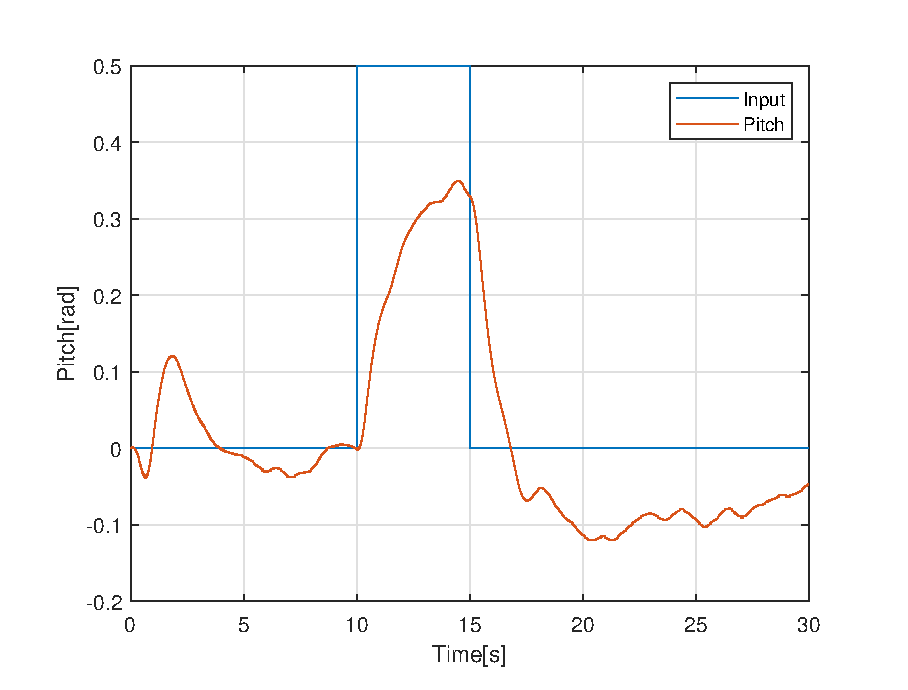
\includegraphics[width=\textwidth]{figures/labday1/-1,-1.eps}
      \caption{Poles at $-1$ and $-1$}
      \label{subfig:poles-1,-1}
    \end{subfigure}

    \begin{subfigure}{0.40\textwidth}
        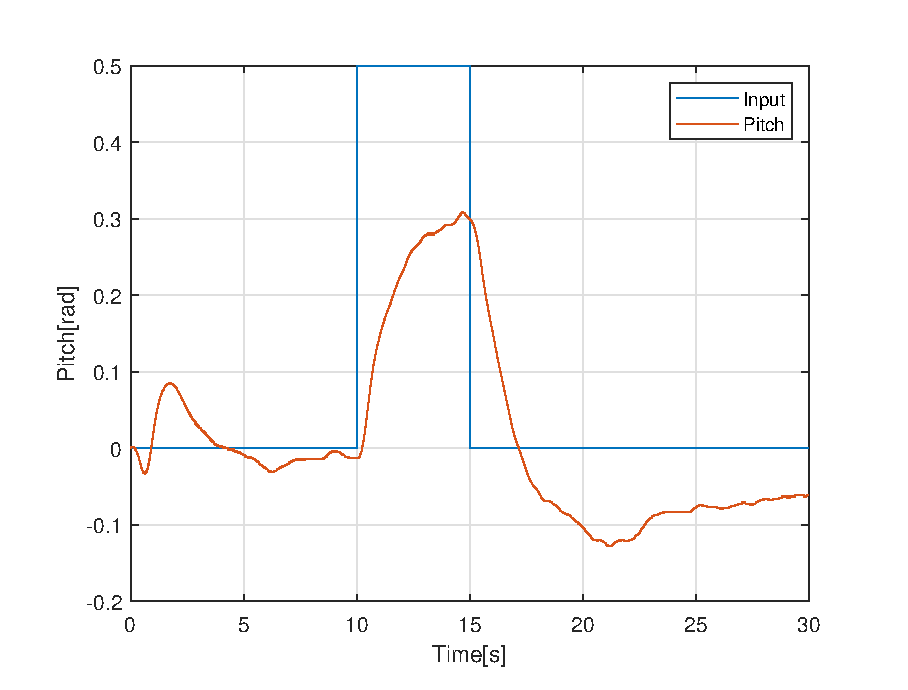
\includegraphics[width=\textwidth]{figures/labday1/-0.5,-2.eps}
        \caption{Poles at $-0.5$ and $-2$.}
        \label{fig:ld1:poles_-0.5,-2}
    \end{subfigure}
    
    \begin{subfigure}{0.40\textwidth}
        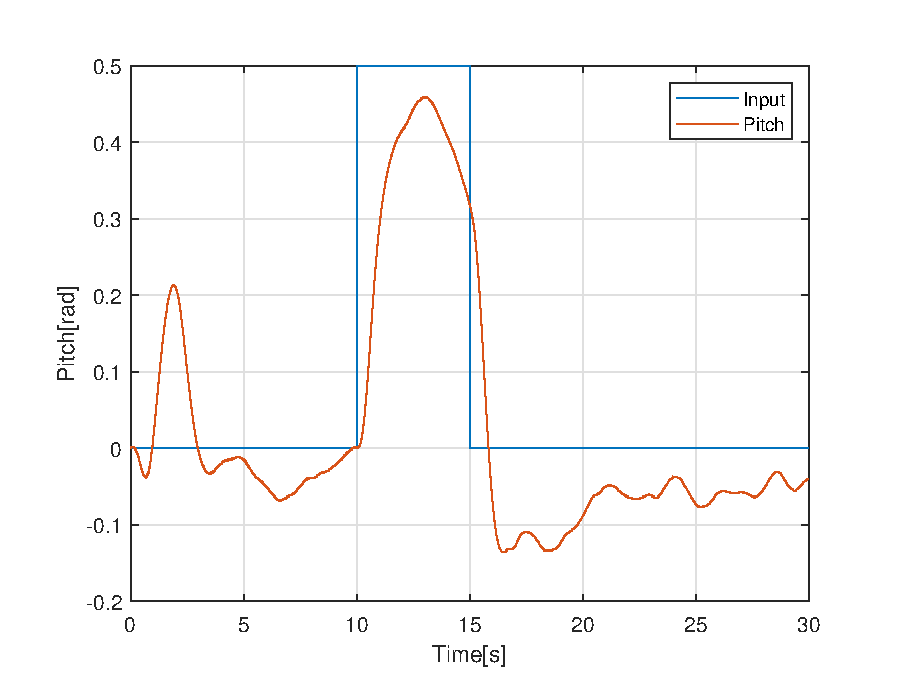
\includegraphics[width=\textwidth]{figures/labday1/-0.5+j,-0.5-j.eps}
        \caption{Poles at $-0.5+j$ and $-0.5 - j$.}
        \label{subfig:ld1:poles_-0.5+j,-0.5-j}
    \end{subfigure}

    \begin{subfigure}{0.40\textwidth}
        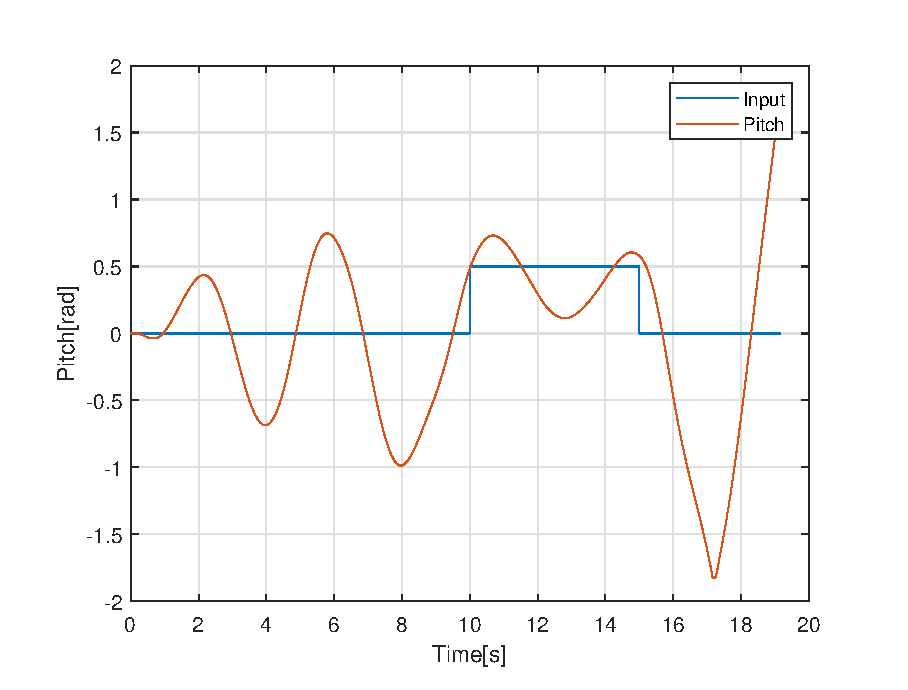
\includegraphics[width=\textwidth]{figures/labday1/j,-j.eps}
        \caption{Poles at $j$ and $-j$}
        \label{fig:ld1:poles_j,-j}   
    \end{subfigure}
        
    \begin{subfigure}{0.40\textwidth}
        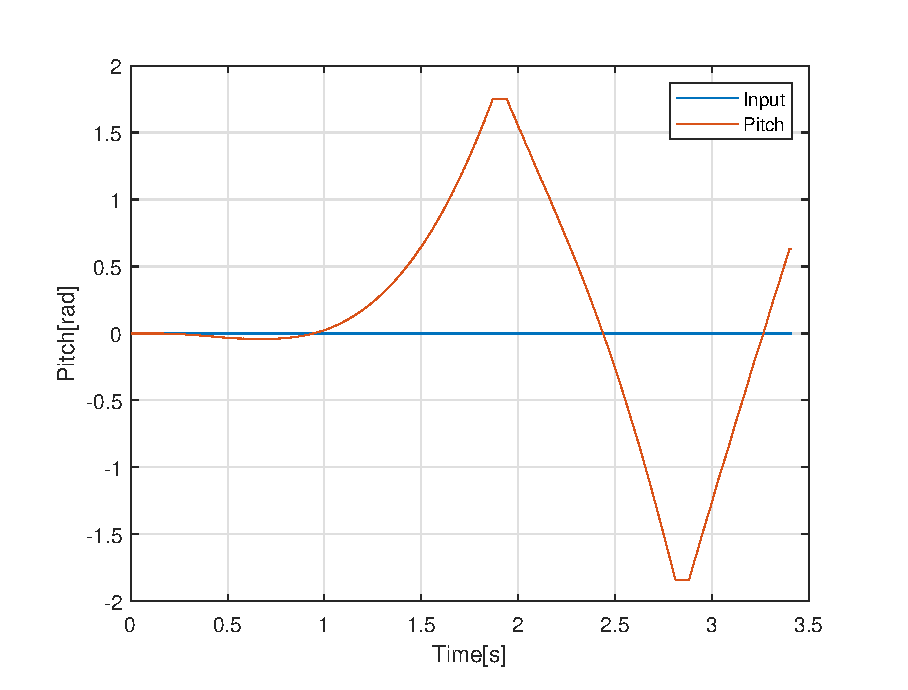
\includegraphics[width=\textwidth]{figures/labday1/1,1.eps}
        \caption{Poles at $1$ and $1$}
    \label{fig:ld1:poles_1,1}
    \end{subfigure}
    
    \caption{Results for different poles}
    \label{fig:labday1resultsdifferentpoles}
    
\end{figure}


\autoref{subfig:poles-1,-1} shows a stable response that rises quickly; however, the system never reaches the target. Indicating a stationary offset. In addition it was not expected that the pitch would go bellow $0$ after the last step function.


\autoref{subfig:ld1:poles_-0.5+j,-0.5-j} shows a response that rises faster than in \autoref{fig:ld1:poles_-1,-1}, and with minimal oscialtions. However these oscilation can be noise.


\autoref{fig:ld1:poles_-0.5,-2} show a response that more slowly reaches the reference. This can be a result of a over dampened system, which is expected with two negative poles at the real axis.



\autoref{fig:ld1:poles_j,-j} shows a response with large oscialtions. The experiment was manually stopped after the helicopter crashed. The expected response is standing oscilations, which almost matches the actual response. However the oscialtions start before the step in the reference, which can be a result of some disturbances in the system. The actual oscialtions was also increasing in amplitude a bit, which led the system to crash, therefore the experiment was stopped a bit early.



\autoref{fig:ld1:poles_1,1} show a unstable plot, where a small disturbance make the pitch increase exponentially. This lead to a fast crash and the experiment was stopped. The result was expected since the poles was in the right half-plane.

Our hypotheses were somewhat right, except that the purely imaginary poles became unstable. Also the fact that poles at $-0.5 +j$ and $0.5 + j$ gave the best response was not expected.